%!TEX root = ../../../_main.tex
\section{Twisted weak ordering algorithms}
\label{sec:twisted-involutions-algorithms}

Now we address the problem of calculating $Wk(\theta)$ for an arbitrary Coxeter group $W$, given in form of a set of generating symbols $S = \{s_1, \ldots s_n\}$ and the relations in form of $m_{ij} = \ord(s_i s_j)$. From this input we want to calculate the Hasse diagram, i.e.\ the vertex set $\ti{\theta}$ and the edges labeled with $\ul s$. Thanks to \ref{lemm:twisted-e-orbit-coincides-with-twisted-involutions} the vertex set can be obtained by walking the $e$-orbit of the action from \ref{defi:twisted-operation}. The only element of twisted length 0 is $e$. Suppose we have already calculated the Hasse diagram until the twisted length $k$, i.e.\ we know all vertices $w \in \ti{\theta}$ with $\rho(w) \leq k$ and all edges connecting two vertices $u,v$ with $\rho(u) + 1 = \rho(v) \leq k$. Let $\rho_k := \{ w \in \ti{\theta} : \rho(w) = k \}$. Then all vertices in $\rho_{k+1}$ are of the form $w \ul s$ for some $w \in \rho_k, s \in S$. For each $(w,s) \in \rho_k \times S$, we calculate $w \ul s$. If $\rho(w \ul s) = k + 1$ then $w \prec w \ul s$. To avoid having to check the twisted length we use \ref{lemm:rho-w-ul-s-minus-rho-w-differs-by-1}. We already know the set $S_w \subseteq S$ of all generators yielding an edge into $w$. Due to the lemma we have $\rho(w \ul s) = k - 1$ for all $s \in S_w$ and $\rho(w \ul s) = k + 1$ for all $s \in S \setminus S_w$. Hence, we only calculate $w \ul s$ for $s \in S \setminus S_w$ and know $w \prec w \ul s$ without checking the twisted length explicitly. The last problem to solve is the possibility of two different $(w,s),(v,t) \in \rho_k \times S$ with $w \ul s = v \ul t$. To deal with this, we have to compare a potential new twisted involution $w \ul s$ with each element of twisted length $k+1$, already calculated. The concrete problem of comparing two elements in a free presented group, called \defword{word problem for groups}, will not be addressed here. We suppose that whatever computer system is used to implement our algorithm, supplies a suitable way to do that. The only thing to note is that solving the word problem is not a cheap operation. Reducing the count of element comparisons is a major demand to any algorithm, calculating $Wk(\theta)$. For a general approach on effective element multiplication in arbitrary Coxeter groups see \cite{casselman:coxeter-multiplication-i,casselman:coxeter-multiplication-ii}.

The steps discussed have been compiled into an algorithm by \cite[Algorithm 2.4]{brennemann:twoa} and \cite[Algorithm 3.1.1]{haas:twoa}. We take this as our starting point. Since the runtime is far from being optimal, we use the structural properties of rank-2-residues from Section \ref{sec:twisted-involutions-residues} to improve the algorithm. As we will show these optimizations yield an algorithm with an asymptotical perfect runtime behavior. \ref{algo:twoa1} and its optimizations have essentially the same structure in common. This is shown in \ref{algo:twoa0}.

\begin{algo}[TWOABase]
	This algorithm takes a Coxeter system $(W,S)$, an involutory Coxeter system automorphism $\theta$ and an upper bound $k_{max}$ for the maximal twisted length to consider as input. It returns the Hasse diagram of $Wk(W,\theta)$ with vertex set $V$ and the set of directed and labled edges $E$.
	\namedlabel{algo:twoa0}
	\begin{algorithmic}[1]
	\Procedure{TwistedWeakOrderingAlgorithmBase}{$(W,S),\theta,k_{max}$} 
	\State $V \gets \{(e,0)\}$
	\State $E \gets \{\}$

	\For{$k \gets 0 \textbf{ to } k_{max}$} \label{algo:twoa0-k-loop}
		\ForAll{$(w,k_w) \in V \textbf{ with } k_w = k$} \label{algo:twoa0-v-loop}
			\ForAll{$s \in S \textbf{ with } \nexists (\cdot,w,s) \in E$} \label{algo:twoa0-s-loop} \Comment{Only for $s \notin D_R(w)$}
				\If{$w \ul s \notin V$} \label{algo:twoa0-decision} \Comment{Check if $w \ul s$ already known}
					\State $V \gets V \cup \{ (w \ul s,k+1) \}$
				\EndIf
				\State $E \gets E \cup \{ (w,w \ul s,l(w \ul s) - l(w)),s \}$
			\EndFor
		\EndFor
		\State $k \gets k + 1$
	\EndFor

	\State \textbf{return} $(V,E)$\Comment{The poset graph}
	\EndProcedure
	\end{algorithmic}
\end{algo}

\begin{rema}
	Note that if $W$ is finite, then we can drop $k_{max}$ and instead use another termination condition: when $k$ reaches the maximal twisted length in $Wk(\theta)$, then the only vertex of twisted length $k$ is the unique element $w_0 \in W$ of maximal ordinary length. Since $s \in D_R(w_0)$ for all $s \in S$, there is no $s' \in S$ remaining to calculate $w_0 \ul s'$ for. This condition can be checked to terminate the algorithm without knowing $k_{max}$ before. When $W$ is infinite, there is no maximal element and $\ti{\theta}$ is infinite, too. In this case $k_{max}$ is used to terminate after having calculated a finite part of $Wk(\theta)$.
\end{rema}

\begin{lemm}
	\typedlabel{lemm:twoa0-algo}
	\ref{algo:twoa0} is a deterministic algorithm if and only if the decision at line~\ref{algo:twoa0-decision} is taken by a deterministic algorithm.

	\begin{proof}
		The outer loop (line \ref{algo:twoa0-k-loop}) is strictly ascending in $k \in \{0,\ldots,k_{max}\}$ and so finite. The innermost loop (line \ref{algo:twoa0-s-loop}) is finite since $S$ is finite and the inner loop (line \ref{algo:twoa0-v-loop}) is finite, since $V$ starts as finite set and in each step there are added at most $|V| \cdot |S|$ many new vertices. Therefore the algorithm terminates. The soundness is due to the arguments at the beginning of Section \ref{sec:twisted-involutions-algorithms}.
	\end{proof}
\end{lemm}

When investigating the asymptotic runtime behavior of our algorithms, we will describe them relative to $k_{max}$ and $n := |\{ w \in \ti{\theta} : \rho(w) \leq k_{max} \}|$ while assuming $\mathcal{O}(|S|) = 1$ and $\mathcal{O}(\ord(st)) = 1$ for all $s,t \in S$ with $\ord(st) < \infty$. We justify this by the fact that the runtime cannot be better than linear in $\mathcal{O}(n)$ (since this is the size of the vertex set $V$ produced by our algorithms) and, moreover, $|S|$ and $\ord(st)$ are tiny in comparison.

\begin{prop}
	\typedlabel{prop:twoa0-runtime}
	Let $A$ be a concrete algorithm instance of \ref{algo:twoa0}. By this we mean an algorithm $A$ that has the form of \ref{algo:twoa0} together with an algorithm $D$ to decide $w \ul s \in V$ at line~\ref{algo:twoa0-decision}. Then for $k = k_{max}$ and $n = |\{ w \in \ti{\theta} : \rho(w) \leq k \}|$ we have $A \in \mathcal{O}(n \cdot D)$.

	\begin{proof}
		The body of the inner loop (line \ref{algo:twoa0-v-loop}) is executed precisely $n$ times and the body contains of $D$ and some instructions with constant runtime.
	\end{proof}
\end{prop}

The poset graph is build up from the unique element of rank 0, the neutral element $e$. Then all elements of rank $1$ are calculated including all edges between elements of rank 0 and rank 1. This is repeated until the rank $k_{max}$ is reached. As we will see, the if-statement at line~\ref{algo:twoa0-decision} in \ref{algo:twoa0} is the crucial point in the algorithm. The naive way of checking $w \ul s \in V$ is to calculate $w \ul s$ as group element in $W$ and then do an element comparison of $w \ul s$ in $W$ with all elements already in $V$ with twisted length $k+1$. This is exactly what \ref{algo:twoa1} does.

\begin{algo}[TWOA1]
	\namedlabel{algo:twoa1}
	\theocite{Algorithm 2.4}{brennemann:twoa}
	\theocite{Algorithm 3.1.1}{haas:twoa}
	This algorithm is based on \ref{algo:twoa0}. It uses the following function to determine if $w \ul s \in V$ at line~\ref{algo:twoa0-decision} in \ref{algo:twoa0}.

	\begin{algorithmic}[1]
	\Procedure{CheckIfAlreadyKnown}{$(W,S),\theta,w,s,V,E$}
		\State $y \gets ws$
		\State $z \gets \theta(s)y$
		\If{$z=w$} \Comment{Explicit element comparison in $W$}
			\State $x \gets y$
		\Else
			\State $x \gets z$
		\EndIf
		
		\ForAll{$(v,k_{v}) \in V \textbf{ with } k_{v} = k+1$} \label{algo:twoa1-comp} \Comment{Check if $x$ already known}
			\If{$x = v$} \Comment{Explicit element comparison}
				\State \textbf{return true}
			\EndIf
		\EndFor
		
		\State \textbf{return false}
	\EndProcedure
	\end{algorithmic}
\end{algo}

\begin{lemm}
	\typedlabel{lemm:twoa1-algo}
	\ref{algo:twoa1} is a deterministic algorithm.

	\begin{proof}
		Since the algorithm for $w \ul s \in V$ just compares $w \ul s$ with all elements in $V$ of same twisted length it is sound. For $k \in \nn_0$ we have $|\{ w \in W : \rho(w) = k \}| < \infty$ and therefore it terminates.
	\end{proof}
\end{lemm}

\begin{lemm}
	\typedlabel{lemm:twoa1-runtime}
	Let $k \in \nn$, $n = |\{ w \in \ti{\theta} : \rho(w) \leq k \}|$. Then \ref{algo:twoa1} $\in \mathcal{O}(n^2/k)$.

	\begin{proof}
		We omit the detailed worst case analysis of \ref{algo:twoa1}. Instead we give an outline of the proof. Let $D$ be the algorithm to check $w \ul s \in V$. When $D$ is executed, then $w \ul s$ is compared to all $w \in V$ with $\rho(w) = k+1$. If $w \ul s$ is the first element of twisted length $k + 1$, then there is nothing to compare. If it is the last element with this twisted length that is not already known, then there are almost as many comparisons needed as elements with this twisted length exist in $\ti{\theta}$. Overall we can assume $D \in \mathcal{O}(n/k)$. By \ref{prop:twoa0-runtime} we get \ref{algo:twoa1} $\in \mathcal{O}(n^2/k)$.
	\end{proof}
\end{lemm}

Any algorithm calculating $Wk(\theta)$ must be at least linear in the size $n$ of the resulting vertice set. Our goal is to improve \ref{algo:twoa1} so that we get an algorithm in $\mathcal{O}(n)$, i.e.\ an asymptotical perfect algorithm for calculating $Wk(\theta)$. As already seen the element comparison of a potential new element with all already known elements of same twisted length (\ref{algo:twoa1} at line~\ref{algo:twoa1-comp}) is the bottleneck. Here the rank-2-residues become key. Suppose we have a $w \in \ti{\theta}$ with $\rho(w) = k$ and $s \in S$. In \ref{algo:twoa1} we would now check if $w \ul s$ is a new vertex or if we already calculated it by comparing it with all already known vertices of twisted length $k + 1$. Assume we have already calculated it. This means there is another twisted involution $v$ with $\rho(v) = k$ and another generator $t \in S$ with $v \ul t = w \ul s$. With \ref{prop:rank-2-residues-are-convex} $w \ul s$ is the unique element of maximal twisted length in the rank-2-residue $wC_{\{s,t\}}$. This yields a necessary condition for $w \ul s$ to be equal to an already known vertex, allowing us to replace the ineffective search all method in \ref{algo:twoa1} at line~\ref{algo:twoa1-comp}.

\begin{figure}[ht]
	\centering
	%!TEX root = ../../_main.tex
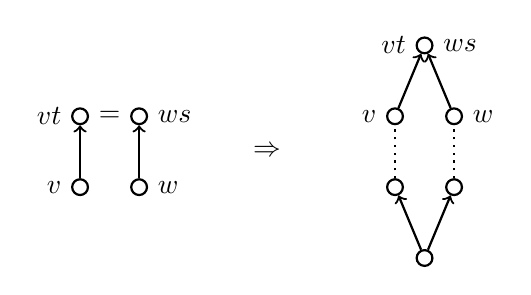
\begin{tikzpicture}[scale=1,bend angle=10]
\newcommand{\xspace}{1}
\newcommand{\yspace}{0.6}
\tikzstyle{vertex}=[draw,thick,circle,minimum size=2mm,inner sep=1pt]
\tikzstyle{edge}=[thick,->]
\tikzstyle{edge2}=[dotted,thick]
\tikzstyle{onesided}=[edge,dashed]
\tikzstyle{bothsided}=[edge]

\node[vertex, label=180:$v$] (3) at (\xspace*-0.375,\yspace*1.5) {};
\node[vertex, label=360:$w$] (4) at (\xspace*0.375,\yspace*1.5) {};
\node[vertex, label=180:$v \ul t$] (5) at (\xspace*-0.375,\yspace*3.0) {};
\node[vertex, label=360:$w \ul s$] (6) at (\xspace*0.375,\yspace*3.0) {};
\node (7) at (\xspace*0,\yspace*3.0) {$=$};
\draw[bothsided] (3) edge (5);
\draw[bothsided] (4) edge (6);

\node (then) at (\xspace*2,\yspace*2.25) {$\Rightarrow$};

\node[vertex] (0) at (4+\xspace*0,\yspace*0) {};
\node[vertex] (1) at (4+\xspace*-0.375,\yspace*1.5) {};
\node[vertex] (2) at (4+\xspace*0.375,\yspace*1.5) {};
\node[vertex, label=180:$v$] (3) at (4+\xspace*-0.375,\yspace*3.0) {};
\node[vertex, label=360:$w$] (4) at (4+\xspace*0.375,\yspace*3.0) {};
\node[vertex, label=180:$v \ul t$, label=360:$w \ul s$] (5) at (4+\xspace*0,\yspace*4.5) {};
\draw[bothsided] (0) edge (1);
\draw[bothsided] (0) edge (2);
\draw[edge2] (1) edge (3);
\draw[edge2] (2) edge (4);
\draw[bothsided] (3) edge (5);
\draw[bothsided] (4) edge (5);
\end{tikzpicture}
	\caption{Optimization of \ref{algo:twoa1}}
	\label{fig:optimization-of-twoa1}
\end{figure}

\begin{prop}
	\typedlabel{prop:twoa1-necessary-condition-for-ws-eq-vt}
	Let $k \in \nn$ and suppose we are in the situation described at the beginning of Section \ref{sec:twisted-involutions-algorithms}. Let $\rho_i := \{ w \in \ti{\theta} : \rho(w) = i \}$ and $\rho'_{k+1}$ the set of the already calculated vertices with twisted length $k+1$. If $w \ul s \in \rho'_{k+1}$ for some $w \in \rho_k, s \in S$, say $w \ul s = v \ul t$ with $v \in \rho_k$ and $t \in S \setminus \{s\}$, then $w \ul s = w[\ul t \ul s]^n$ for some $n \in \nn$ with $w[\ul t \ul s]^j \in \rho_0 \cup \ldots \cup \rho_k \cup \rho'_{k+1}$ for $1 \leq j \leq n$.

	\begin{proof}
		The equality $w \ul s = w[\ul t \ul s]^n$ for some $n \in \nn$ is due to \ref{prop:rank-2-residues-are-convex}. All vertices in this rank-2-residue except $v \ul t$ have a twisted length of $k$ or lower. For $v \ul t$ we supposed it is already known, hence $v \ul t \in \rho'_{k+1}$. Therefore all vertices $w[\ul t \ul s]^j$, $1 \leq j \leq n$ are in $\rho_0 \cup \ldots \cup \rho_k \cup \rho'_{k+1}$.
	\end{proof}
\end{prop}

This can be checked effectively. Both, $w$ and $s$ are fixed. Start with $M = \emptyset$. For all already known edges from or to $w$ being labeled with $\ul t \in \ul S \setminus \{\ul s\}$ we do the following: walk $w[\ul t \ul s]^i$ for $i = 0,1,\ldots$ until $\rho(w[\ul t \ul s]^i) = k + 1$. Note that walking in this case really means walking the graph. All involved vertices and edges have already been calculated. So there is no need for more calculations in $W$ to find $w[\ul t \ul s]^i$. By \ref{prop:rank-2-residues-are-convex} such a path must exist (in a completely calculated graph). But we could be in the case, where the last step from $w[\ul t \ul s]^{i-1}$ to $w[\ul t \ul s]^{i}$ has not been calculated yet. If it is already calculated, then add this element to $M$ by setting $M = M \cup \{ w[\ul t \ul s]^{i} \}$. If not, do not add it to $M$.

Now $M$ contains all already known elements of twisted length $k+1$, satisfying the necessary condition from \ref{prop:twoa1-necessary-condition-for-ws-eq-vt}. Furthermore, $|M| < |S|$. So for each pair $(w,s)$ we have to do at most $|S|-1$ many element comparisons the determine if $w \ul s$ is new or already known, no matter how many elements of twisted length $k+1$ are already known. This can be used to massively improve \ref{algo:twoa1}.

\begin{algo}[TWOA2]
	\namedlabel{algo:twoa2}
	This algorithm is based on \ref{algo:twoa0}. It uses the following function to determine if $w \ul s \in V$ at line~\ref{algo:twoa0-decision} in \ref{algo:twoa0}.

	\begin{algorithmic}[1]
	\Procedure{CheckIfAlreadyKnown}{$(W,S),\theta,w,s,V,E$}
		\State $y \gets ws$
		\State $z \gets \theta(s)y$
		\If{$z=w$} \Comment{Explicit element comparison in $W$}
			\State $x \gets y$
		\Else
			\State $x \gets z$
		\EndIf

		\ForAll{$t \in S \setminus \{S\}$} \label{algo:twoa2-s-loop}
			\If{$\ord(st) < \infty$}
				\State $v \gets w$
				\State $k \gets 1$
				\State $(z_0,z_1) \gets (s,t)$

				\While{\textbf{true}} \label{algo:twoa2-height-loop-down} \Comment{Walk $wC_{\{s,t\}} \cap V$ down}
					\State $e \gets (v_0,v_1,a,l) \in E \textrm{ with } v_1 = v \textrm{ and } a = z_{k \mod 2}$

					\If{$e = \textbf{null}$}
						\State \textbf{break}
					\EndIf

					\State $v \gets v_0$
					\State $k \gets k + 1$
				\EndWhile

				\While{\textbf{true}} \label{algo:twoa2-height-loop-up} \Comment{Walk $wC_{\{s,t\}} \cap V$ up the other branch}
					\State $e \gets (v_0,v_1,a,l) \in E \textrm{ with } v_0 = v \textrm{ and } a = z_{k \mod 2}$

					\If{$e = \textbf{null}$}
						\State \textbf{break}
					\EndIf

					\State $v \gets v_1$
					\State $k \gets k - 1$
				\EndWhile

				\If{k = 0} \Comment{Check if $\rho(v) = \rho(w) + 1$}
					\If{$x = v$} \Comment{Explicit element comparison in $W$}
						\State \textbf{return true}
					\EndIf
				\EndIf
			\EndIf
		\EndFor

		\State \textbf{return false}
	\EndProcedure
	\end{algorithmic}
\end{algo}

\begin{lemm}
	\typedlabel{lemm:twoa2-algo}
	\ref{algo:twoa2} is a deterministic algorithm.

	\begin{proof}
		The outer loop (line~\ref{algo:twoa2-s-loop}) is executed $|S|-1$ times. Its body is only called if $\ord(st)$ is finite. Due to \ref{lemm:max-twisted-circle-height} both inner while loops (lines~\ref{algo:twoa2-height-loop-down},\ref{algo:twoa2-height-loop-up}) are executed at most $2 \cdot \ord(st)$ times. So \ref{algo:twoa2} terminates. The soundness of this improvement is due to \ref{prop:twoa1-necessary-condition-for-ws-eq-vt}.
	\end{proof}
\end{lemm}

\begin{lemm}
	\typedlabel{lemm:twoa2-runtime}
	Let $k \in \nn$, $n = |\{ w \in \ti{\theta} : \rho(w) \leq k \}|$. Then $\ref{algo:twoa2} \in \mathcal{O}(n)$.

	\begin{proof}
		Let $D$ be the algorithm to check $w \ul s \in V$. As seen in the proof of \ref{lemm:twoa2-algo}, the execution count for each while loop in $D$ does not exceed
		$$ (|S|-1) \cdot \max \{ \ord(st) : t \in S \setminus \{s\}, \ord(st) < \infty \}. $$
		Since we considered $|S|$ and $\ord(st)$ constant we have $D \in \mathcal{O}(1)$ and so with \ref{prop:twoa0-runtime} we have \ref{algo:twoa2} $\in \mathcal{O}(n)$. 
	\end{proof}
\end{lemm}

Many more explicit element comparisons can be avoided. In some cases we can deduce the equality $v \ul t = w \ul s$ as well as $l(w \ul s) - l(w)$ just from the already calculated structure of the rank-2-residue $wC_{\{s,t\}}$, while in other cases we can preclude that $v \ul t$ equals $w \ul s$. The following two corollaries show examples of restrictions that rank-2-residues are subjected to:

\begin{coro}
	Let $w \in \ti{\theta}$ with $\rho(w) = k$, $s,t$ be two distinct generators and $s \notin D_R(w)$. Suppose $n \in \nn$ to be the smallest number for that $\rho(w[\ul t \ul s]^{2n-1}) = k + 1$ holds. Then:

	\begin{enumerate}
		\item If $n = \ord(st)$, then $w[\ul t \ul s]^{2n-1} = w \ul s$.
		\item If $n \geq 2$ and $l(w[\ul t \ul s]^{2n-1}) - l(w[\ul t \ul s]^{2n-2}) = 1$, then $w[\ul t \ul s]^{2n-1} = w \ul s$.
	\end{enumerate}

	\begin{proof}

		\begin{enumerate}
			\item Follows immediately from \ref{lemm:max-twisted-circle-height}.
			\item Because of the length difference the step from $w[\ul t \ul s]^{2n-2}$ to $w[\ul t \ul s]^{2n-1}$ is a multiplication, not a twisted conjugation, and because of $n \geq 1$ this step cannot be next to the smallest element in $wC_{\{s,t\}}$. Hence, $w[\ul t \ul s]^{2n-1} = w \ul s$ by \ref{coro:onesided-operations-only-at-top-or-bottom-end-of-twocycle}. \qedhere
		\end{enumerate}
	\end{proof}
\end{coro}

\begin{coro}
	Let $w \in S$ and $s,t \in S$ be two distinct generators. Then the following table shows all possible $n \in \nn$ with $w(\ul s \ul t)^n = w$ regarding $\ord(st)$ and the distribution of multiplications and twisted conjugations in $wC_{\{s,t\}}$ (see Figure~\ref{fig:dist-one-bothsided-actions-in-rank-2-residue}).

	\begin{center}
		\begin{tabular}{c|ccccccc|c}
													& \multicolumn{7}{c|}{$\ord(st)$} \\
													& 2 & 3 & 4 & 5 & 6 & 7 & 8 \\
			\hline
			\textrm{non-multiplicative}				& 1,2 & 3 & 2,4 & 5 & 2,3,4,6 & 7 & 2,4,6,8 \\
			\textrm{diagonal-multiplicative}		& 2 & 3 & 2,4 & 5 & 2,3,4,6 & 7 & 2,4,6,8 \\
			\textrm{maximal-multiplicative}			& 2 & -- & 3 & -- & 2,4 & -- & 5 \\
			\textrm{bottom- and top-multiplicative}	& -- & 2 & -- & 3 & -- & 2,4 & -- \\
		\end{tabular}		
	\end{center}

	\begin{proof}
		In each case we get a $m$ with $w = (\ul s \ul t)^m$ by \ref{lemm:max-twisted-circle-height} and \ref{lemm:max-rank-2-residue-size-special-cases}. By \ref{coro:rank-2-residue-gcd-n-m} any $n$ with this property has a non trivial divisor in common with $m$ if $w \ul s \neq w \ul t$. The situation $w \ul s \ul t = w$ for $s \neq t$ can only occur if $\ord(st) = 2$ and if $\ul s$ and $\ul t$ act by twisted conjugation on $w$ due to \ref{lemm:double-edges-only-for-ord-2} and the proof of \ref{lemm:no-triple-edges}.
	\end{proof}
\end{coro}

We use these restrictions to further improve \ref{algo:twoa2}:

\begin{prop}
	\typedlabel{prop:twoa3-decision-tree}
	Let $w \in \ti{\theta}$ with $\rho(w) = k$, $s,t \in S$ be two distinct generators with $m := \ord(st) < \infty$ and $n \in \nn$ the smallest number with $\rho(w[\ul t \ul s]^n) = k+1$. Note that $n$ has to be odd in this case. We define $v := w[\ul t \ul s]^{n-1}$, $h := (n+1)/2$ and
	\begin{align*}
		a_1 & = l(w \ul s) - l(w) - 1, \\
		a_2 & = l(w[\ul t \ul s]^{h-1}) - l(w[\ul t \ul s]^{h-2}) - 1, \\
		a_3 & = l(w[\ul t \ul s]^{h}) - l(w[\ul t \ul s]^{h-1}) - 1 \textrm{ and} \\
		a_4 & = l(w[\ul t \ul s]^{2h-1}) - l(w[\ul t \ul s]^{2h-2}) - 1.
	\end{align*}
	Then the following decision tree allows to decide if $v \ul t = w \ul s$ or not in many cases.

	\begin{enumerate}
		\item $h=1$:
			\begin{enumerate}
				\item $m=2$:
					\begin{enumerate}
						\item $a_4=1$:
							Maybe $v \ul t = w \ul s$. If it is the case, then $a_1 = 1$.
						\item $a_4=0$:
							Then $v \ul t \neq w \ul s$.
					\end{enumerate}
				\item $m>2$:
					Then $v \ul t \neq w \ul s$.
			\end{enumerate}
		\item $h>1$:
			\begin{enumerate}
				\item $a_4=0$:
					Then $v \ul t = w \ul s$ and $a_1 = a_3 + a_4 - a_2$.
				\item $(a_2,a_3)=(1,1)$:
					\begin{enumerate}
						\item $h=m$: Then $v \ul t = w \ul s$ and $a_1 = 1$.
						\item $\gcd(h,m)>1$: Maybe $v \ul t = w \ul s$. If it is the case, then $a_1 = 1$.
						\item $\textrm{else}$: Then $v \ul t \neq w \ul s$.
					\end{enumerate}
				\item $(a_2,a_3)=(1,0)$:
					\begin{enumerate}
						\item $h=m$: Then $v \ul t = w \ul s$ and $a_1 = 0$.
						\item $\gcd(h,m)>1$: Maybe $v \ul t = w \ul s$. If it is the case, then $a_1 = 0$.
						\item $\textrm{else}$: Then $v \ul t \neq w \ul s$.
					\end{enumerate}
				\item $(a_2,a_3)=(0,0)$:
					\begin{enumerate}
						\item $h=(m+1)/2$: Then $v \ul t = w \ul s$ and $a_1 = 1$.
						\item $\gcd(h,(m+1)/2)>1$: Maybe $v \ul t = w \ul s$. If it is the case, then $a_1 = 1$.
						\item $\textrm{else}$: Then $v \ul t \neq w \ul s$.
					\end{enumerate}
			\end{enumerate}
	\end{enumerate}

	\begin{proof}
		First of all we convince ourselves that this decision tree is complete. This is immediate, since by $h \geq 0$, $m \geq 2$ and \ref{prop:one-both-sided-action-symmetric-in-rank-2-residues}. Suppose $h=1$. This means $v = w$. In case $v \ul t = w \ul s$, then we have a double edge between $w$ and $w \ul s$. By \ref{lemm:double-edges-only-for-ord-2} this is possible only if $m = \ord(st) = 2$ and $a_4 = l(w \ul t) - l(w) - 1 = 1$. Now suppose $h > 1$ and $a_4=0$. By \ref{lemm:onesided-operations-only-at-top-or-bottom-end-of-twocycle} either $v \ul s \succ v$ or $v \ul t \ul s \prec v \ul t$. Since $h > 1$ we cannot have $v \ul s \succ v$, hence $v \ul t \ul s \prec v \ul t$. Then $v \ul t$ is the unique maximal element in $wC_{\{s,t\}}$ and so $w \ul s = v \ul t$. Now suppose $h > 1$ and $a_4=1$ and furthermore suppose $(a_2,a_3)=(1,1)$ (the other cases are analogue). If $h = m$, then by \ref{lemm:max-twisted-circle-height} $v \ul t$ is again the unique maximal element and $v \ul t = w \ul s$. If $h < m$ then by \ref{coro:rank-2-residue-gcd-n-m} $v \ul t = w \ul s$ is only possible if $\gcd(h,m) > 1$. In all cases the deduction of $a_1$ is possible with \ref{prop:deduction-of-s-action-in-rank-2-residue}.
	\end{proof}
\end{prop}

\begin{algo}[TWOA3]
	\namedlabel{algo:twoa3}
	In general this algorithm proceeds like \ref{algo:twoa2}. But instead of comparing $w \ul s$ with the list of all possible already known elements $v \ul t$, it uses the decision tree from \ref{prop:twoa3-decision-tree} to either directly find $v \ul t$ with $v \ul t = w \ul s$ or at least to sort out elements from the list that cannot be equal to $w \ul s$. The information needed for the decision tree, namely $w, s, t, h, a_2, a_3, a_4$ (cf. \ref{prop:twoa3-decision-tree}), can easily be extracted, when searching for the already calculated elements $v \ul t$ with $\rho(v \ul t) = \rho(w) + 1$. This algorithm then applies the decision tree to each of them to decide if $w \ul s = v \ul t$, or if $w \ul s \neq v \ul t$ or if explicit element comparison is needed, to get a final answer to this question. We will omit the concrete details and refer to the appendix, where an implementation of this algorithm can be found.
\end{algo}

\begin{lemm}
	\typedlabel{lemm:twoa3-algo}
	\ref{algo:twoa3} is a deterministic algorithm.

	\begin{proof}
		By construction, \ref{algo:twoa3} has the same loops as \ref{algo:twoa2}, which is a deterministic algorithm. In addition \ref{algo:twoa3} uses the decision tree from \ref{prop:twoa3-decision-tree}. Since the decision tree has no loops, is terminates and we have already proved its correctness. Hence \ref{algo:twoa3} is correct and it terminates.
	\end{proof}
\end{lemm}

\begin{lemm}
	\typedlabel{lemm:twoa3-runtime}
	Let $k \in \nn$, $n = |\{ w \in \ti{\theta} : \rho(w) \leq k \}|$. Then $\ref{algo:twoa3} \in \mathcal{O}(n)$.

	\begin{proof}
		Since the decision tree has constant runtime the asymptotical runtime of \ref{algo:twoa3} cannot be worse than the asymptotical runtime of \ref{algo:twoa2}.
	\end{proof}
\end{lemm}